%-----------------------------------------------------
% Conclusion
%-----------------------------------------------------
\newpage

\section{Conclusion}
The main results of this study are as follows:
\begin{enumerate} 
	\item
	
\begin{figure}[h!]
		\begin{center}
			\begin{tabular}{cc}
				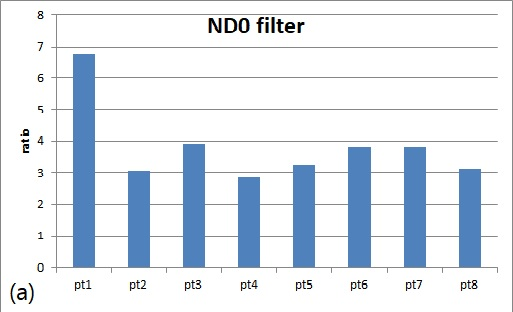
\includegraphics[width=7cm]{ND0} &
				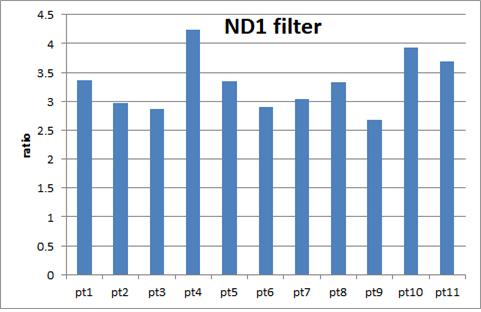
\includegraphics[width=7cm]{ND1}
			\end{tabular}
			\caption{The histogram shows the ratio between exciton recombination rate and biexcitonrate, differed by the point of laser. Left picture is when ND0 filter is used, and the right picture is when ND1 filter is used.The standard deviation of ratio is 0.432 and 0.483, respectively. }	
			\label{fig:FIR221}
		\end{center}
	\end{figure}
	Exciton recombination rate와 biexciton recombination rate 사이의 비율의 평균은 3.43와 3.30이었다. 이론적으로 알려진 2.29이라는 비율\cite{chen2018room} 과는 다소 상이하였으나 두 속도 사이의 비율이 결정의 위치가 바뀌어도 일정한 것으로 보아 만들어진 결정이 동일한 특성을 지닌 물질이라는 것을 확인 할 수 있었다.  
	\item 
	
	
	\item It is possible to detect more outflows by using a higher energy emission line of $^{12}$CO. Using data with smaller beamwidth also enhances detecting outflows. The reason that higher energy lines can detect more outflows can be explained as the following. The excitation temperature is higher for emission lines with higher energy. Outflows drag out matter from the protostar's envelope, which has higher temperature than its surroundings. Lines with higher energy are emitted, which has an effect that makes column density higher than usual.	
\end{enumerate}